\appendix
\part{Appendices}
\label{part:appendices}

\chapter{Appendix for Chapter \ref{chap:effective-analysis}}
\label{chap:appendix-effective-analysis}

% Keep prompt-box settings local to this appendix.
\begingroup
\tcbset{autoparskip}

\section{Additional Related Work}
\start{Analyses on the Effectiveness of General Agent Training} 
Outside SWE, Agent-FLAN~\citep{chen2024agentflan} shows that agent corpora entangle format following with reasoning and redesigns them to separate the two. With regard to reasoning, the structure and behaviors of a trace matter more than its correctness: with verification, backtracking, and related behaviors, RL would be able to gain even from incorrect solutions~\citep{gandhi2025cognitive}, and long-CoT distillation tolerates wrong answers but not shuffled or deleted steps~\citep{li2025structure}. Furthermore, \citet{beneficial-reasoning} find the same for agentic search, where SFT on trajectories exhibiting beneficial behaviors before RL outperforms SFT on outcome-correct ones. 




\section{Experimental Setup}
\label{catradar:sec:analysis-setup}
\start{Datasets and Models}
We conduct evaluation on the SWE-bench Verified dataset~\citep{swebench} and analysis on both in-domain training: the R2E-Gym issue-solving dataset~\citep{R2EGym}, and transfer learning: the Hybrid-Gym function localization dataset~\citep{hybrid-gym}. 
We experiment on 3 student models: Qwen2.5Coder-7B~\citep{qwen25coder}, Qwen3-4B, and Qwen3-8B~\citep{qwen3} and 8 teacher models: Claude-Opus-4.5~\citep{claude45}, Claude-Opus-4.7~\citep{claude47}, Claude-Sonnet-3.5~\citep{claude35}, GPT-5-mini~\citep{gpt5}, GPT-5.5~\citep{gpt55}, DeepSeek4-flash~\citep{deepseekv4}, Qwen3-80B~\citep{qwen3}, and Qwen3.5-397B~\citep{qwen35}.

\start{Training Details}
We fine-tune each student on the teacher demonstrations with supervised fine-tuning: we use 8 A6000 GPUs and search hyper-parameters in the range of learning-rate=\{5e-5, 1e-4\}, num-epochs=\{3, 5\}, and batch-size=\{8, 16\}.


\start{Training and Evaluation Prompts}
All Hybrid-Gym teacher rollouts use the function localization prompt in \autoref{catradar:fig:prompt-funcloc}, which asks for a single function or class, except the strategy-prompted rollouts in \S\ref{catradar:sec:exp-implementation}.
The students are evaluated on SWE-Bench Verified~\cite{swebench} with the issue-solving prompt in \autoref{catradar:fig:prompt-issue}.
On R2E-Gym, whose images come with a ready virtual environment instead of conda, the Claude-Sonnet-3.5 rollouts come from the original R2EGym dataset and use the original R2E-Gym prompt~\citep{R2EGym} (\autoref{catradar:fig:prompt-r2egym}). Other models use the same prompt as our SWE-Bench Verified evaluation.


\vspace{0.4cm}
\begin{tcolorbox}[colback=gray!5!white,colframe=gray!75!black,title=Function Localization Prompt,fontupper={\scriptsize\ttfamily\rightskip=0pt plus 1fil},breakable,break at=-36pt]

I've uploaded a python code repository in the directory \{\{ workspace\_dir\_name \}\}.\\
Your goal is to locate the \{\{ module\_type \}\} described below and write its docstring.\\
\\
<\{\{ module\_type \}\}\_description>\\
\{\{ description \}\}\\
</\{\{ module\_type \}\}\_description>\\
\\
Known details:\\
- Target type: \{\{ module\_type \}\}\\
- The original docstring was removed; please restore/author it.\\
- Note: The target name is not provided. You must identify the correct \{\{ module\_type \}\} based on the functionality description above.\\
\\
Follow these steps:\\
1. EXPLORATION: Search the codebase (no file path provided) to find where this \{\{ module\_type \}\} is defined.\\
2. UNDERSTANDING: Read the implementation to fully understand its arguments, return values, and side effects.\\
3. RECHECK: Verify that the \{\{ module\_type \}\} you located actually matches the given description. Compare the implementation behavior with the description to ensure you found the correct target.\\
4. GENERATION: Insert a clear, concise Python docstring inside the definition using triple quotes. Cover purpose, parameters, return value(s), and important behaviors or exceptions.\\
5. REVIEW: Double-check formatting and accuracy; avoid changing code outside the docstring unless strictly necessary.\\
Be thorough in your exploration and reasoning. It's fine if your thinking process is lengthy - quality and completeness are more important than brevity.
\end{tcolorbox}
\captionof{figure}{The Hybrid-Gym function localization prompt. \texttt{module\_type} is \texttt{function} or \texttt{class}.}
\label{catradar:fig:prompt-funcloc}


\begin{tcolorbox}[colback=gray!5!white,colframe=gray!75!black,title=Original R2E-Gym Prompt,fontupper={\scriptsize\ttfamily\rightskip=0pt plus 1fil},breakable,break at=-36pt]
Consider the following github issue:\\
<github\_issue>\\
\{\{ instance.problem\_statement \}\}\\
</github\_issue>\\
\\
Can you help me implement the necessary changes to the repository to fix the <github\_issue>?\\
I've already taken care of all changes to any of the test files described in the <github\_issue>. This means you DON'T have to modify the testing logic or any of the tests in any way!\\
Your task is to make the minimal changes to non-tests files in the /testbed directory to ensure the <github\_issue> is satisfied.\\
\\
IMPORTANT TIP:\\
Follow these steps to resolve the issue:\\
1. As a first step, it might be a good idea to explore the repo to familiarize yourself with its structure.\\
2. Create a script ('reproduce\_issue.py') to reproduce the error and execute it to confirm the error\\
3. Edit the sourcecode of the repo to resolve the issue\\
4. Rerun your reproduce script and confirm that the error is fixed!\\
5. Think about edgecases and make sure your fix handles them as well
\end{tcolorbox}
\captionof{figure}{The R2E-Gym prompt~\citep{R2EGym}, used by some of the R2E-Gym rollouts.}
\label{catradar:fig:prompt-r2egym}

\clearpage

\begin{tcolorbox}[colback=gray!5!white,colframe=gray!75!black,title=Issue-Solving Prompt,fontupper={\scriptsize\ttfamily\rightskip=0pt plus 1fil},breakable]
I have access to a python code repository in the directory \{\{ instance.repo\_path \}\} . You can explore and modify files using the available tools. Consider the following issue description:\\
\\
<issue\_description>\\
\{\{ instance.problem\_statement \}\}\\
</issue\_description>\\
\\
Can you help me implement the necessary changes to the repository so that the requirements specified in the <issue\_description> are met?\\
I've already taken care of all changes to any of the test files described in the <issue\_description>. This means you DON'T have to modify the testing logic or any of the tests in any way!\\
Also the development Python environment is already set up for you (i.e., all dependencies already installed), so you don't need to install other packages.\\
Your task is to make the minimal changes to non-test files in the \{\{ instance.repo\_path \}\} directory to ensure the <issue\_description> is satisfied.\\
\\
Follow these phases to resolve the issue:\\
\\
Phase 1. READING: read the problem and reword it in clearer terms\\
~~~1.1 If there are code or config snippets. Express in words any best practices or conventions in them.\\
~~~1.2 Hightlight message errors, method names, variables, file names, stack traces, and technical details.\\
~~~1.3 Explain the problem in clear terms.\\
~~~1.4 Enumerate the steps to reproduce the problem.\\
~~~1.5 Hightlight any best practices to take into account when testing and fixing the issue\\
\\
Phase 2. RUNNING: install and run the tests on the repository\\
~~~2.1 Activate the environment by running\\
~~~~~~~./opt/miniconda3/etc/profile.d/conda.sh ; conda activate testbed\\
~~~2.2 Follow the readme\\
~~~2.3 Install the environment and anything needed\\
~~~2.4 Iterate and figure out how to run the tests\\
\\
Phase 3. EXPLORATION: find the files that are related to the problem and possible solutions\\
~~~3.1 Use `grep` to search for relevant methods, classes, keywords and error messages.\\
~~~3.2 Identify all files related to the problem statement.\\
~~~3.3 Propose the methods and files to fix the issue and explain why.\\
~~~3.4 From the possible file locations, select the most likely location to fix the issue.\\
\\
Phase 4. TEST CREATION: before implementing any fix, create a script to reproduce and verify the issue.\\
~~~4.1 Look at existing test files in the repository to understand the test format/structure.\\
~~~4.2 Create a minimal reproduction script that reproduces the located issue.\\
~~~4.3 Run the reproduction script to confirm you are reproducing the issue.\\
~~~4.4 Adjust the reproduction script as necessary.\\
\\
Phase 5. FIX ANALYSIS: state clearly the problem and how to fix it\\
~~~5.1 State clearly what the problem is.\\
~~~5.2 State clearly where the problem is located.\\
~~~5.3 State clearly how the test reproduces the issue.\\
~~~5.4 State clearly the best practices to take into account in the fix.\\
~~~5.5 State clearly how to fix the problem.\\
\\
Phase 6. FIX IMPLEMENTATION: Edit the source code to implement your chosen solution.\\
~~~6.1 Make minimal, focused changes to fix the issue.\\
\\
Phase 7. VERIFICATION: Test your implementation thoroughly.\\
~~~7.1 Run your reproduction script to verify the fix works.\\
~~~7.2 Add edge cases to your test script to ensure comprehensive coverage.\\
~~~7.3 Run existing tests related to the modified code to ensure you haven't broken anything.\\
\\
8. FINAL REVIEW: Carefully re-read the problem description and compare your changes with the base commit \{\{ instance.base\_commit \}\}.\\
~~~8.1 Ensure you've fully addressed all requirements.\\
~~~8.2 Run any tests in the repository related to:\\
~~~~~8.2.1 The issue you are fixing\\
~~~~~8.2.2 The files you modified\\
~~~~~8.2.3 The functions you changed\\
~~~8.3 If any tests fail, revise your implementation until all tests pass\\
\\
Be thorough in your exploration, testing, and reasoning. It's fine if your thinking process is lengthy - quality and completeness are more important than brevity.
\end{tcolorbox}
\captionof{figure}{The issue-solving prompt used to evaluate the students on SWE-Bench Verified and used in some of the R2E-Gym rollouts.}
\label{catradar:fig:prompt-issue}



\clearpage

\section{Computation of Significance}
With the paired bootstrap test of \citet{berg-kirkpatrick-etal-2012-empirical}, we test whether two students differ in resolved rate on SWE-Bench Verified.
Let $\delta(x)$ be the gain in resolved rate of the better student over the other on the 500 instances $x$.
We draw $b=10^6$ samples $x^{(i)}$ of 500 instances from $x$ with replacement and estimate the one-sided p-value as the fraction of samples with $\delta(x^{(i)}) \geq 2\delta(x)$; the threshold is $2\delta(x)$ rather than $\delta(x)$ because the samples are centered at $\delta(x)$ instead of at 0.
We mark a change as significant if $p<0.05$.


\section{List of Candidate Behaviors}
\label{catradar:sec:full-candidate-behaviors}
In \autoref{catradar:tab:distinct-behaviors-full-list}, we provide a list of candidate behaviors on which we do not conduct further experiments. The reason is that we prioritize the behaviors that are more likely to be useful for training.




\section{Detailed Analysis Results}
\subsection{Exploration Length is Not a Good Indicator of Trajectory Effectiveness}
Following \S\ref{catradar:sec:traj-features}, we show that the exploration length of demonstrations is, however, not a good indicator of trajectory effectiveness.

\begin{figure}[h]
    \centering
        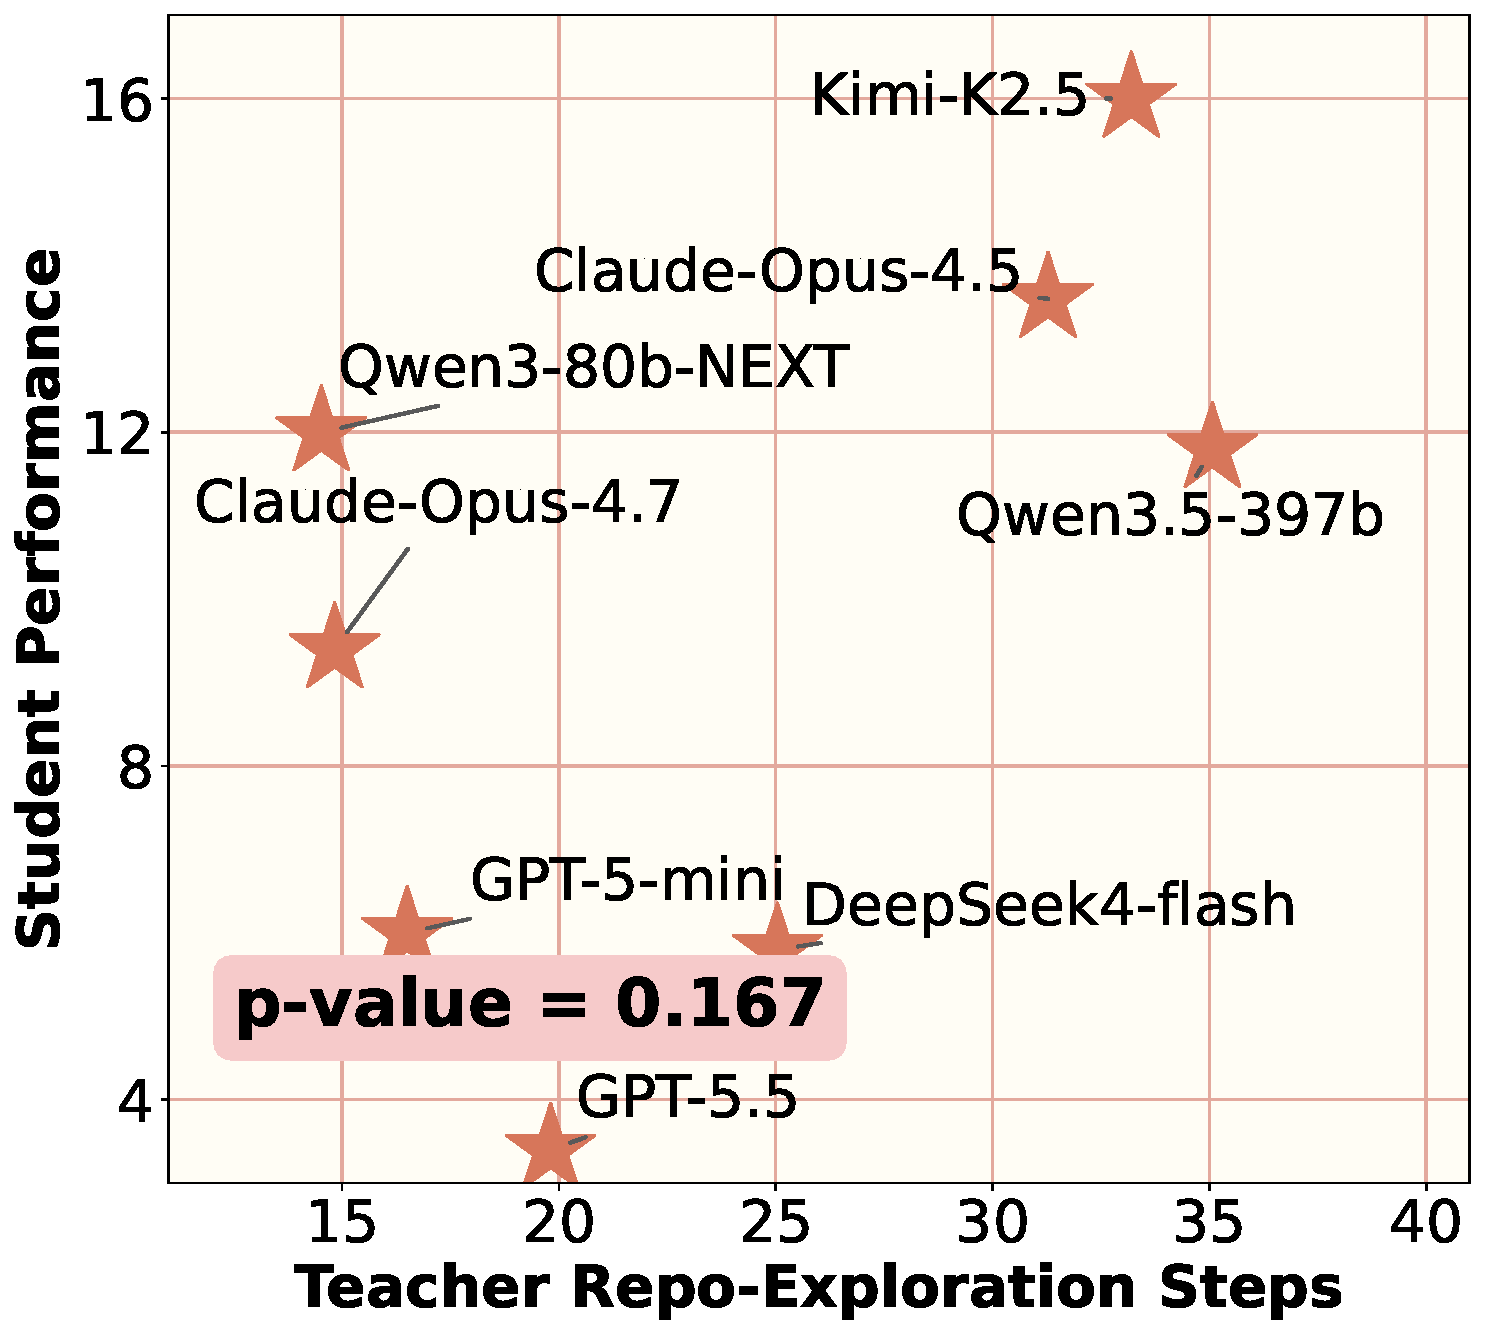
\includegraphics[width=\linewidth,height=3.6cm,keepaspectratio]{CATRadar_figs/agent_behaviors/teacher_expo_len_student_acc.pdf}
    \caption{The exploration length of demonstrations is also not a good indicator of demonstration effectiveness.}
    \label{catradar:fig:exp-len-correlation}
\end{figure}



\subsection{Strong Teacher Does Not Always Translate to Strong Student}
Some Claude-Opus-4.7 demonstrations open the target file without saying why they chose it, as is shown in \autoref{catradar:tab:skip-case}.
On an instance that asks for a class with ``attributes [...] such as their nickname, username, and hostname'', Claude-Opus-4.7 lists the repository's Python files, cut at 50 by \texttt{head}, and then opens the 9th entry, the target file, saying only ``The file \texttt{sopel/tools/target.py} looks promising.''; it runs no content search such as \texttt{grep} and does not narrow the listing in any form.
In other words, the trajectory itself does not show any reason why it picks the target file out of the 50 searched results.
In comparison, Claude-Opus-4.5 has a clearer strategy for file localization.
It first names four candidate files with a reason each, and it checks where the class is used before editing it.
Similarly, for function localization, on \texttt{open-mmlab\_\_mmengine-304\_415}, Claude-Opus-4.7 likewise opens the 44th entry of a 50-file listing (``The class description matches \texttt{base\_model.py}.''), while Claude-Opus-4.5 first lists the six requirements of the description and browses two directories.


\begin{table*}[!t]
    \centering
    \resizebox{0.8\linewidth}{!}{
    \begin{tabular}{>{\raggedright\arraybackslash}m{4.5cm} >{\raggedright\arraybackslash}m{10cm}}
        \toprule
        \bf Behavior & \bf Judge Metric \\
        \midrule
        Search frequency & The frequency of search ($\geq$ 15: high; 7--14: medium; $<$ 7: low) \\

        Search-view ratio & The ratio of keyword searching to file-viewing commands is $> 3$\\
        Multi-round file view & Run file-viewing actions for $\geq 3$ times\\
        Start with thinking & Use the \texttt{\textless function=think\textgreater} tool as the first action \\
        Start with task-tracker & Use the \texttt{\textless function=task\_tracker\textgreater} tool as the first action \\
        Frequent command chain & Use command chaining on 50\% or more of terminal commands \\
        View file before edit & Has a file-viewing action before the first file-editing action \\
        Use Git commands & Use \texttt{git log}, \texttt{git diff}, or other Git commands \\
        \bottomrule
    \end{tabular}
    }
    \caption{The candidate behaviors discovered by \toolName that we do not conduct further experiments on.}
    \label{catradar:tab:distinct-behaviors-full-list}
\end{table*}

\begin{table*}[!t]
    \centering
    \small
    \begin{tabular}{@{}r@{\enspace}>{\raggedright\arraybackslash}p{0.43\linewidth}@{\quad}r@{\enspace}>{\raggedright\arraybackslash}p{0.43\linewidth}@{}}
        \toprule
        \multicolumn{2}{@{}l}{\bf Claude-Opus-4.7 (5 actions)} & \multicolumn{2}{l@{}}{\bf Claude-Opus-4.5 (16 actions)} \\
        \midrule
        1 & \texttt{find <repo> -type f -name "*.py" | head -50 \&\& ls <repo>} $\rightarrow$ 50 file paths (listing cut by \texttt{head}) & 1 & \texttt{view /workspace} $\rightarrow$ directory tree \\
        2 & ``The file \texttt{sopel/tools/target.py} looks promising. Let me check it.'' \texttt{view sopel/tools/target.py} $\rightarrow$ \textcolor{textGreen}{\bf target class \texttt{User}} & 2 & \texttt{view sopel/} $\rightarrow$ directory tree \\
        3 & \texttt{str\_replace}: add the docstring to \texttt{User} & 3 & \texttt{think}: ``[...] this sounds like a User class in an IRC context. Let me look at relevant files: 1.~\texttt{sopel/tools/target.py} - the name `target' could represent users/channels 2.~\texttt{sopel/trigger.py} - might contain user-related classes 3.~\texttt{sopel/bot.py} - could contain user tracking classes 4.~\texttt{sopel/irc.py} - IRC-specific classes'' \\
        4 & \texttt{python -c "from sopel.tools.target import User; print(User.\_\_doc\_\_)"} & 4 & \texttt{view sopel/tools/target.py} $\rightarrow$ \textcolor{textGreen}{\bf target class \texttt{User}} \\
        5 & \texttt{finish} & 5 & \texttt{think}: ``I found the \texttt{User} class [...]'' \\
         & & 6 & \texttt{grep} for the modules that import \texttt{User} \\
         & & 7--8 & \texttt{view sopel/bot.py}, \texttt{view sopel/coretasks.py} \\
         & & 9 & \texttt{think}: ``Now I'm certain the \texttt{User} class [...] is the correct target.'' \\
         & & 10 & \texttt{str\_replace}: add the docstring to \texttt{User} \\
         & & 11--16 & view the edited file, import check, run the test suite (3 commands), \texttt{finish} \\
        \bottomrule
    \end{tabular}
    \caption{Demonstrations of Claude-Opus-4.7 and Claude-Opus-4.5 on the Hybrid-Gym instance \texttt{sopel-irc\_\_sopel-1344\_101} (both successful). \texttt{<repo>} abbreviates the repository path, and file paths are shown relative to it. Claude-Opus-4.7 opens the target file directly from a listing cut at 50 files, while Claude-Opus-4.5 takes a more comprehensive strategy: picking several candidate files with detailed reasoning, and then reading them one-by-one (action 3).}
    \label{catradar:tab:skip-case}
\end{table*}


\subsection{Non-Tool-Call Text Increases Trajectory Length}
Similar to \S\ref{catradar:sec:verbosity}, we observe that when we only increase the verbosity of non-tool call text, the trajectory length in general increases, but the performance doesn't change much.


\begin{figure}[!t]
    \centering
        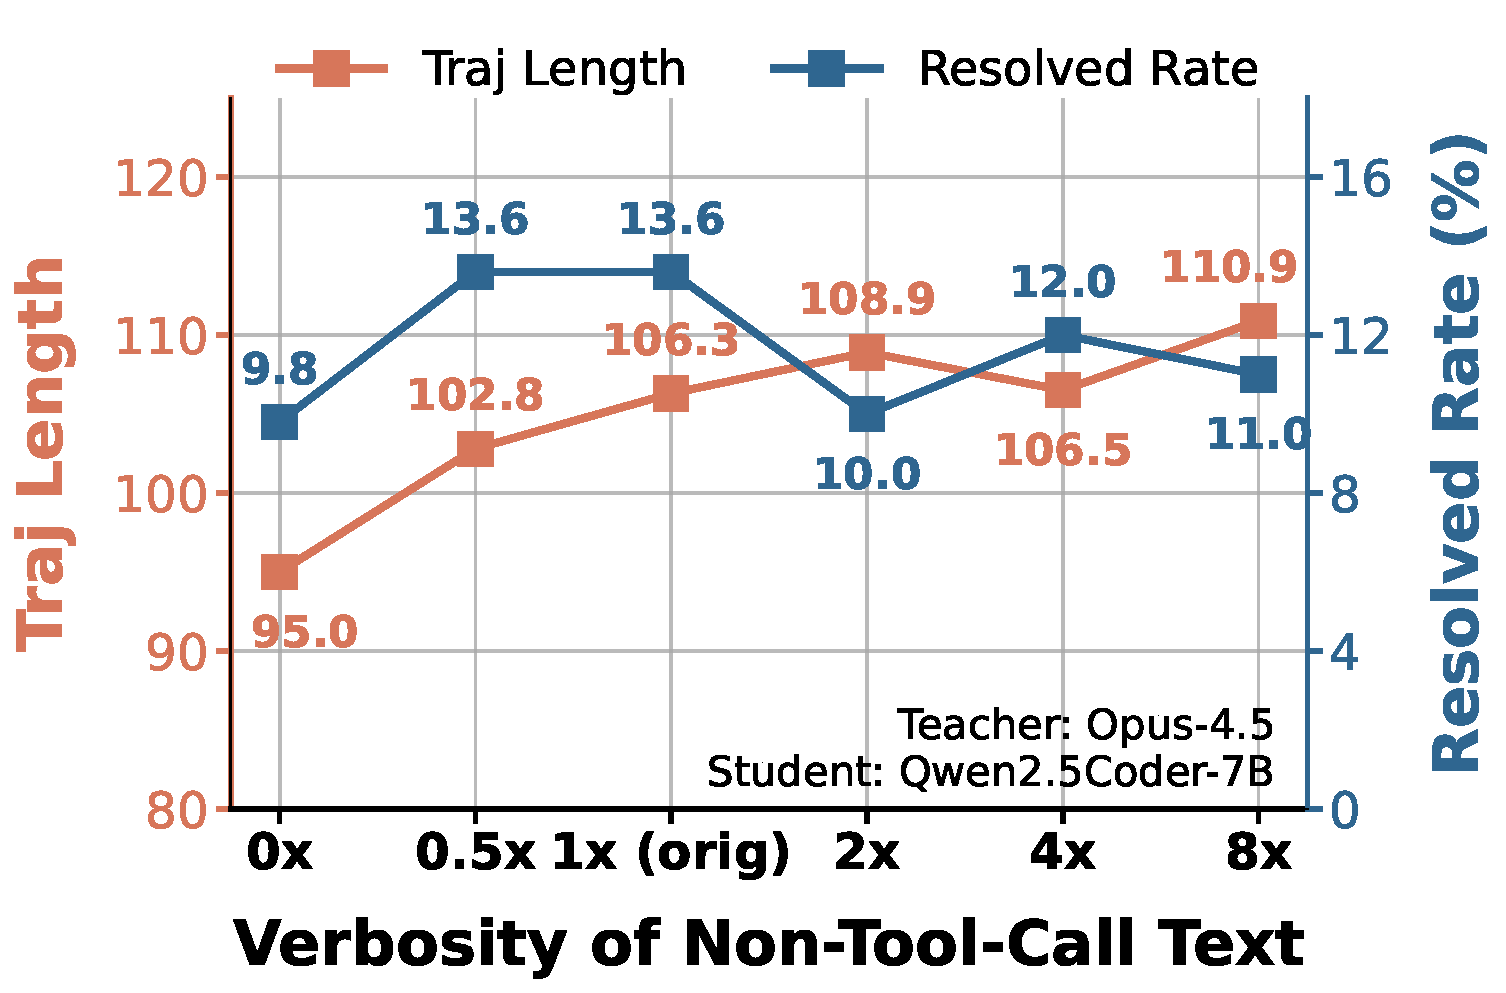
\includegraphics[width=0.8\linewidth]{CATRadar_figs/agent_behaviors/verbosity_text_only.pdf}
    \caption{When we increase the verbosity of non-tool call text, the trajectory length in general increases. However, the performance does not change much.}
    \label{catradar:fig:verbosity_text_only}
\end{figure}

\section{Concrete Data Intervention Implementation for each Candidate Behavior}
\label{catradar:sec:exp-implementation}
In this section, we introduce how we design experiments to control the presence or absence of each candidate behavior in training demonstrations. 
We manually design different experiments for different behaviors.

\subsection{Label Demonstrations with the Presence of Repo-Exploration Strategies}
We label the two strategies with rule-based judges.

\start{Multi-Search}
We define keyword search as a \texttt{terminal} command that contains \texttt{grep} or \texttt{rg}, or \texttt{find} with \texttt{-name}.
A trajectory exhibits the ``Multi-Search'' behavior if it runs at least two keyword searches before its first file-editing action (\texttt{file\_editor} with \texttt{create}, \texttt{str\_replace}, or \texttt{insert}, or a \texttt{sed -i} or \texttt{git apply} command).

\start{Target-Read}
We take the first action that is a \texttt{file\_editor view} (of a file or a directory), a \texttt{terminal} command that contains \texttt{cat}, \texttt{head}, \texttt{tail}, \texttt{less}, or \texttt{more}, or a file-editing action.
Its path is the \texttt{file\_editor} path, or the first argument after \texttt{cat}, \texttt{head}, \texttt{tail}, \texttt{less}, or \texttt{more} in the command.
The trajectory exhibits Target-Read if an earlier keyword search lists at most 30 distinct files and its output contains this path: a listed path equals it, ends with it, or is a suffix of it, has the same file name, or the path or its file name occurs in the output text.




\subsection{Prompt the Models to Adopt our Repo-Exploration Strategies}
This section introduces the experimental settings for the ``prompt teacher'' and ``prompt student'' ablations in \autoref{catradar:tab:prompt-tuning}.

\start{Prompt Teacher}
To instruct the teacher to follow the strategies for the Hybrid-Gym function localization task, we add the \texttt{<localization\_strategy>} block in \autoref{catradar:fig:prompt-strategy} after the steps of the function localization prompt (\autoref{catradar:fig:prompt-funcloc}) and end step~1 with ``Use the localization strategy below.''
GPT-5-mini produces 1,289 successful demonstrations with this prompt, which keep the strategy block in their task prompt. 
It produces 1,346 successful demonstrations with the original prompt (i.e., without the strategy block).
We train the student on all 1,289 demonstrations and evaluate it with the unchanged issue-solving prompt (\autoref{catradar:fig:prompt-issue}).

\start{Prompt Student}
As for the ``prompt student'' ablation, we train the student model on the original 1,346 GPT-5-mini demonstrations.
In inference, we insert the \texttt{<repo\_exploration\_strategy>} block in \autoref{catradar:fig:prompt-strategy} in the prompt for the SWE-Bench Verified issue-solving task, which states the same principles for issue solving, after Phase~3 (EXPLORATION) of the issue-solving prompt at evaluation time.

\begin{figure*}[!t]
\begin{tcolorbox}[colback=gray!5!white,colframe=gray!75!black,title=Strategy Block for the Teacher,fontupper=\small\ttfamily]
<localization\_strategy>\\
When searching for the target \{\{ module\_type \}\}, follow these two principles\\
(summarized from successful trajectories):\\
\\
1. MULTI-ROUND REFINEMENT. Treat localization as iterative. After each\\
~~~search, look at the matches as a whole, pick the most promising signal,\\
~~~and run a follow-up search refining on it (different keyword, restricted\\
~~~path, different surrounding pattern). Do not commit to a single candidate\\
~~~on the first search -- expect 2-3 rounds of refinement before you have a\\
~~~short list.\\
\\
2. READ AFTER NARROWING. Do not open and read full file contents until you\\
~~~have narrowed to a small handful (<=3) of plausible candidates. Opening\\
~~~files too early wastes context on irrelevant code. Once you have a short\\
~~~list, then read each candidate's definition and compare against the\\
~~~description to pick the correct one.\\
</localization\_strategy>
\end{tcolorbox}
\begin{tcolorbox}[colback=gray!5!white,colframe=gray!75!black,title=Strategy Block for the Student,fontupper=\small\ttfamily]
<repo\_exploration\_strategy>\\
When searching the repository for the file(s)/function(s) relevant to the issue,\\
follow these two principles (summarized from successful trajectories):\\
\\
1. MULTI-ROUND REFINEMENT. Treat localization as iterative. After each search,\\
~~~look at the matches as a whole, pick the most promising signal, and run a\\
~~~follow-up search refining on it (different keyword, restricted path, different\\
~~~surrounding pattern). Do not commit to a single candidate on the first search --\\
~~~expect 2-3 rounds of refinement before you have a short list.\\
\\
2. READ AFTER NARROWING. Do not open and read full file contents until you have\\
~~~narrowed to a small handful (<=3) of plausible candidates. Opening files too\\
~~~early wastes context on irrelevant code. Once you have a short list, read each\\
~~~candidate's definition and compare against the issue description to pick the\\
~~~correct one.\\
</repo\_exploration\_strategy>
\end{tcolorbox}
\caption{The strategy blocks added to the teacher's function localization prompt (first box; \texttt{module\_type} is \texttt{function} or \texttt{class}) and to the student's issue-solving prompt (second box).}
\label{catradar:fig:prompt-strategy}
\end{figure*}




\subsection{Add Task-Tracker Steps to Training Demonstrations}
Neither Claude-Opus-4.7 nor GPT-5-mini uses any task-tracker tool calls in its original Hybrid-Gym demonstrations.
To implement the ``Add Task-Tracker'' ablation,
we insert LLM-synthesized task-tracker plans at four points of each demonstration:
(1) before the first action;
(2) once the target file is found, i.e., before the last action prior to the first edit that mentions the target file (the file of the last successful edit);
(3) before the first file-editing action; and
(4) right after the output of the first file-editing action.
If two points coincide, only the earlier point's plan is inserted.
Each plan is a task-tracker action with \texttt{command=plan}, followed by the tool's usual output, ``Task list has been updated with $N$ item(s).''

We use an LLM (DeepSeek4-flash, \citet{deepseekv4}) to write the plans at temperature 0.3 without seeing the demonstration: the first plan from the task description, asked to list 4--6 tasks with the first one in progress, and each later plan from the task description and the first plan, asked to keep the task titles and update their status.
For GPT-5-mini, 1,325 demonstrations receive four plan turns and 21 receive three, and every planning step is consistent with the remaining part of the trajectory.
For Claude-Opus-4.7, 1,466 demonstrations receive four plan turns and one receives three.
However, we cut off 354 of these turns because they change task titles in a later plan item, or generate too few or too many plans in the first task-planner tool call.


\subsection{Add Verification Steps to Training Demonstrations}
As introduced in \S\ref{catradar:sec:verification}, we take the verification steps from Claude-Opus-4.5, whose demonstrations contain more of them (\autoref{catradar:tab:verification-ablation}).
For each Claude-Opus-4.7 demonstration whose instance also has a successful Claude-Opus-4.5 demonstration that first edits the same file (the same path relative to the repository root), we keep the Claude-Opus-4.7 trajectory before its first file-editing action and append the Claude-Opus-4.5 trajectory from its first file-editing action on, with the workspace directory renamed.
That is to say, we copy both the file-editing steps and verification steps from Claude-Opus-4.5's trajectories for the consistency of trajectories.
This applies to 1,389 of the 1,467 demonstrations. We keep the remaining 78 unchanged.


\subsection{Verbosity Experiments}
We use DeepSeek4-flash (with thinking disabled)~\cite{deepseekv4} to rewrite the Claude-Opus-4.5 demonstrations of Hybrid-Gym, which have 30,615 assistant turns, including 3,738 \texttt{think} and 683 task-tracker actions.

For every multiple $k>0$, only the reasoning text changes: every tool call apart from the \texttt{thought} parameter of \texttt{think} calls, and every tool output, stays byte-identical, which we verify on the released datasets.

\start{Non-tool-call text} For \autoref{catradar:fig:verbosity_text_only}, we rewrite the text before the tool call to $k$ times its own length in Qwen3 tokens, for $k\in\{0.5,2,4,8\}$, in every turn except \texttt{think} and task-tracker turns.
10,513 of these 26,194 turns have text; the others, including 4 with a malformed tool call, stay unchanged.
The rewriter sees only the turn's text and its tool call and is told to keep the meaning and intent, not to invent facts, findings, file contents, or results that the text and the call do not imply, and to write as the agent at this step: longer ablations elaborate on what the agent is looking for, why, and what it expects to learn, without adding steps or discoveries; shorter ablations condense the same content.

Different ablations of a turn are written as a ladder in one request: the $0.5\times$ ablation condenses the original, the $2\times$ ablation elaborates it, and the $4\times$ and $8\times$ ablations each elaborate the previous one.
Furthermore, an ablation is accepted if its length is within $\pm 25\%$ of the target; otherwise it is requested again with its measured length as feedback, for at most three rounds, after which the turn keeps its original text, as do turns whose target is below 4 or above 2,000 tokens.

On average, the rewritten texts are 0.5, 1.9, 3.9, and 8.1 times as long as the originals.
Out of the 10,513 turns with text, 0.8\%, 1.3\%, 3.0\%, and 4.1\% keep their original text in the first release described below. The second release has the same rounded rates except at $8\times$ (4.2\%).

The $0\times$ variant removes the text of all turns except the \texttt{think} and task-tracker turns.

\start{Thinking Content} 
For \autoref{catradar:fig:verbosity}, we also rewrite the \texttt{thought} parameter of each \texttt{think} call, and the text before the call, to the same multiple of its own length; the other turns are as in the non-tool-call setting with the same $k$.
The rules for thoughts are the same, adapted to the agent's reasoning: keep its reasoning, conclusions, and concrete references (files, functions, line numbers), and reach no new conclusions or plan different steps.
Thoughts in the trajectories are long (median 304 tokens), so every ablation above 600 tokens is written in several parts, each continuing the text so far, up to 8,000 tokens.
The $0\times$ variant removes all \texttt{think} actions with their outputs and the text of all other turns except the task-tracker turns, which stay whole (99 of them have text).

\start{Post-Checks}
We do not check the meaning of the rewrites.
Instead, we check: 
(1) whether the rewriting describes the rewriting task instead of the agent's reasoning (e.g., ``the thought doesn't mention testing, so I won't plan that''; 4.6\%, 10.0\%, and 19.8\% of the thoughts at $2\times$, $4\times$, and $8\times$) or ended with JSON left from the rewriter's reply (3.3\% of the rewritten $2\times$ and $4\times$ texts);
(2) whether the written reasoning text is natural and consistent with the remaining part of the trajectory.
We keep the original reasoning text if the rewriting does not meet any of the requirements.

\clearpage
\endgroup

\chapter{Appendix for Chapter \ref{chap:critique-training}}
\label{chap:appendix-critique-training}

\begingroup
% Imported from appendix_analysis.tex
\section{Analyses on the Gap between Teacher and Student Critic Models}
\label{critic:app:analyses}
\start{Error Categorization Results}
We first compute the agreement of error categorization between the student and teacher critic models. As shown in \autoref{critic:fig:analysis_error_cat}, the agreement rate is high for major error categories such as step repetition (F1=$0.91$) and task derailment (F1=$0.73$).
The overall average Micro-F1 score is $0.74$.

\start{Overall Guidance Quality}
Then we prompt an LLM judge to check whether the guidance generated by both the teacher and student models is both correct and well-specified.
We use a different model (\texttt{DeepSeek V4 Pro}) as the judge to avoid self-bias.
The results are shown in \autoref{critic:fig:analysis_guidance}, the SFT critic model has a significantly lower rate of generating correct and well-specified guidance compared to the teacher critic model.


\begin{figure*}[t]
    \centering
    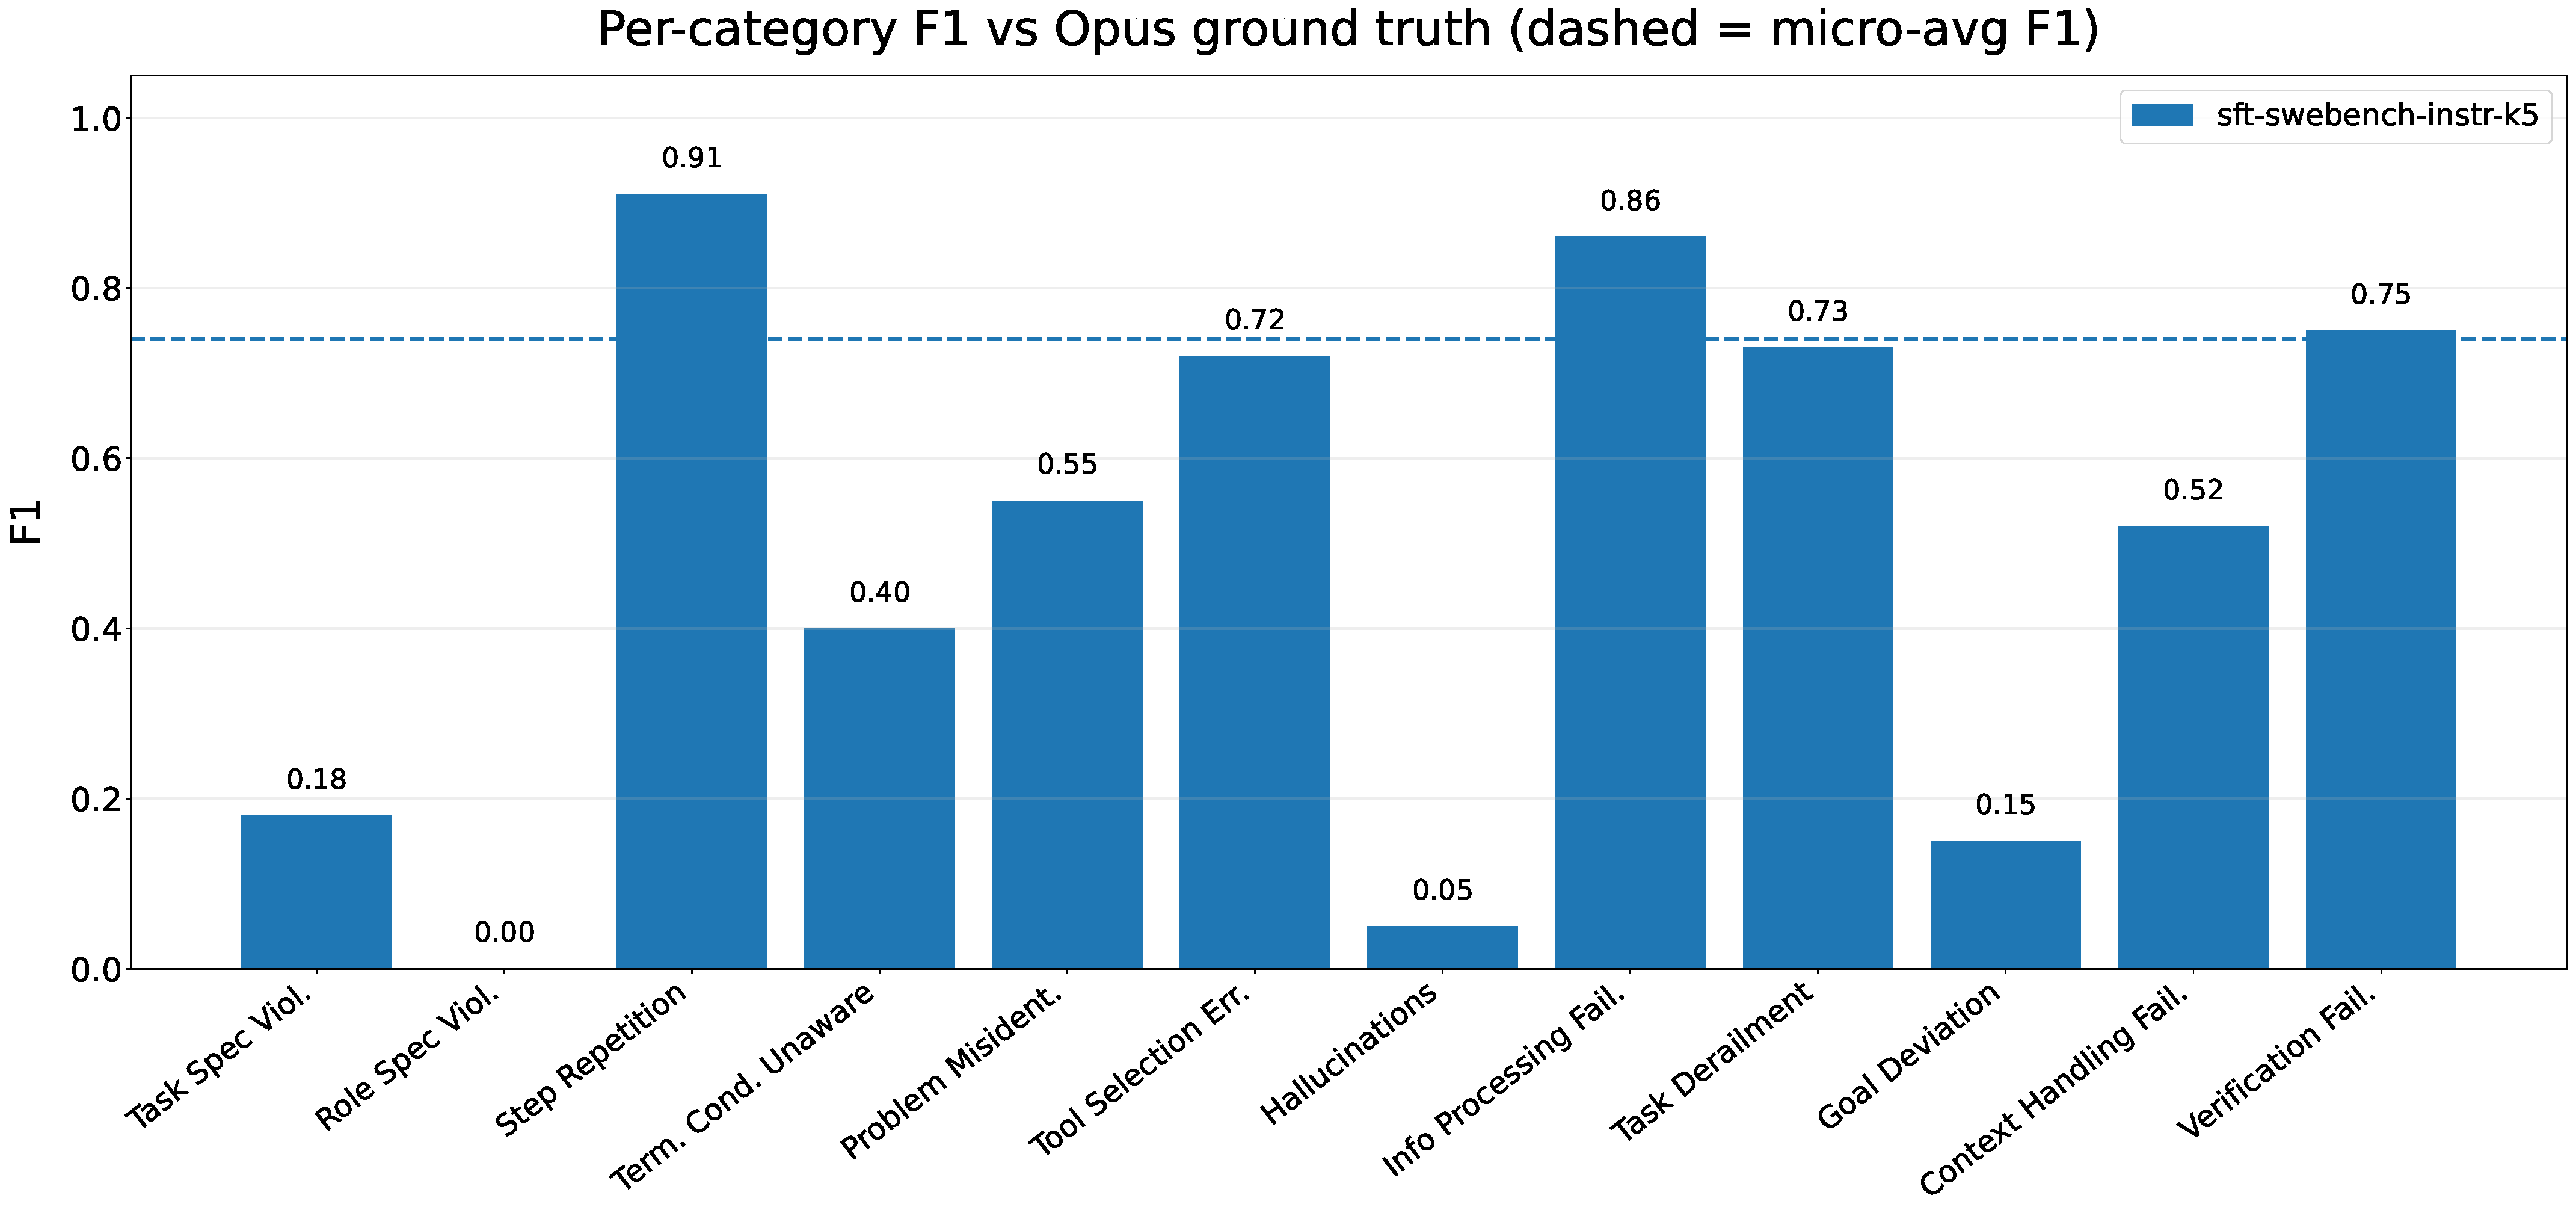
\includegraphics[width=\linewidth]{Critic_figs/analysis_categorization.pdf}
    \caption{Error categorization results.}
    \label{critic:fig:analysis_error_cat}
\end{figure*}

\begin{figure*}[t]
    \centering
    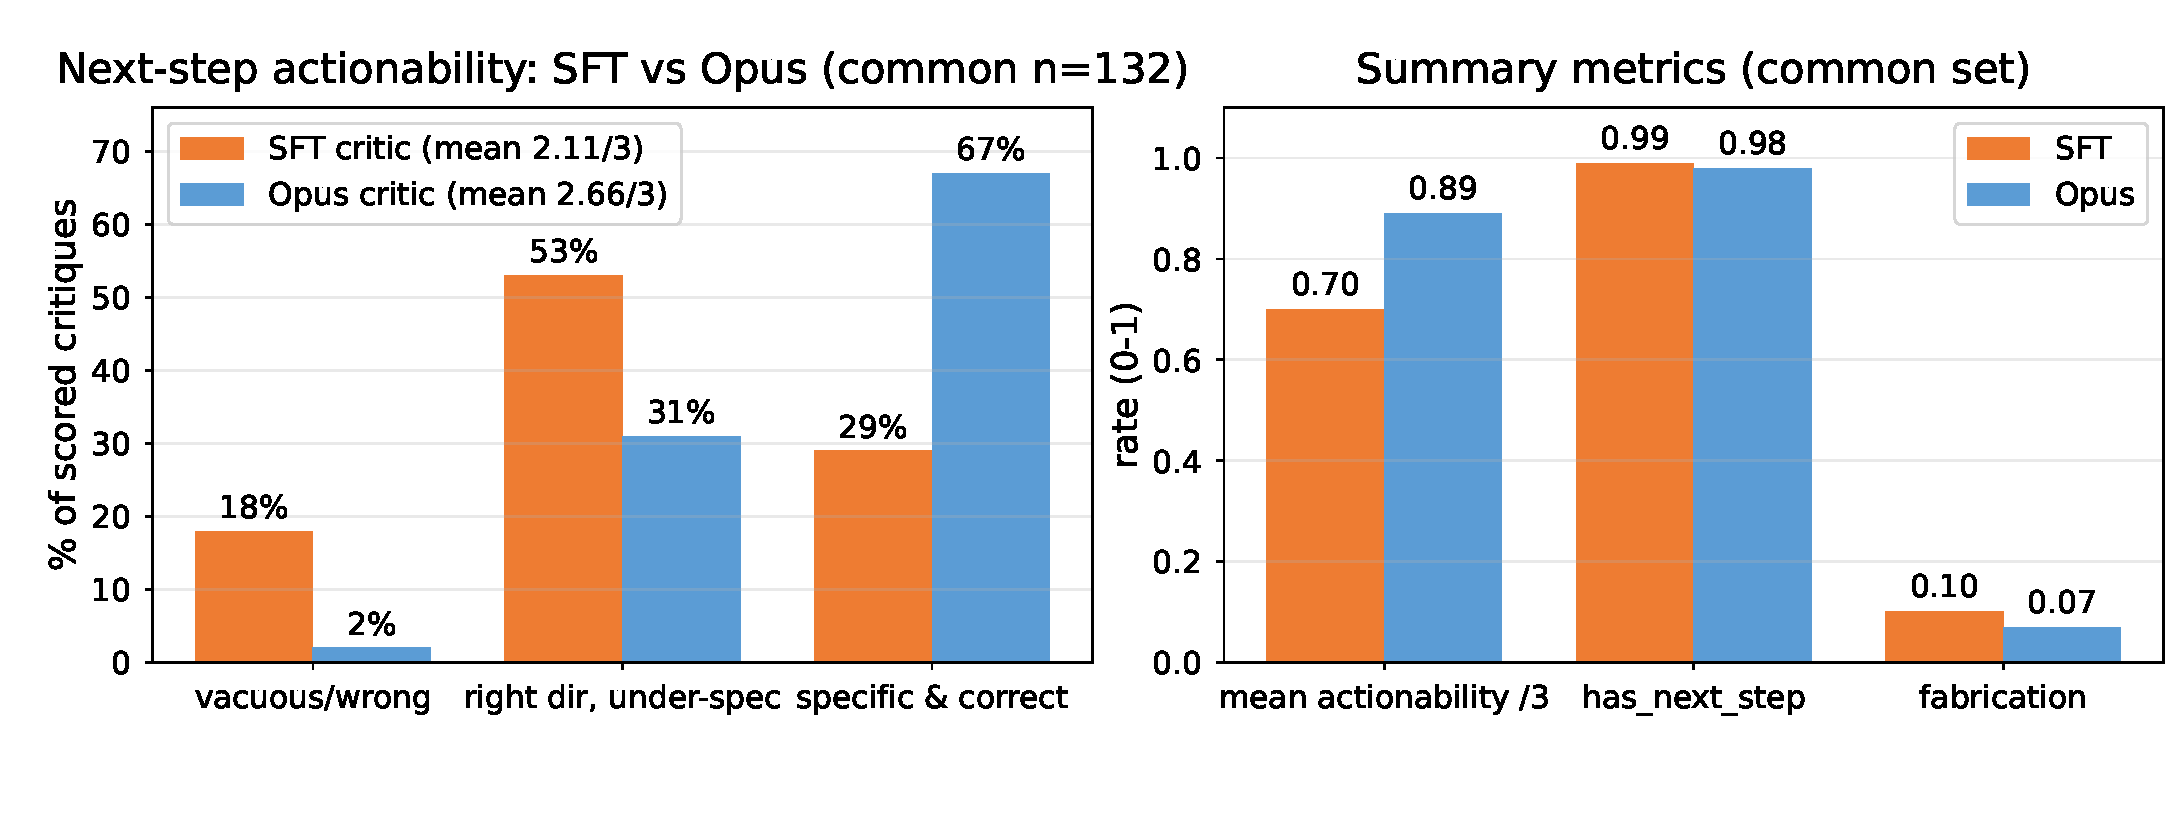
\includegraphics[width=\linewidth]{Critic_figs/analysis_guidance.pdf}
    \caption{Guidance quality analysis.}
    \label{critic:fig:analysis_guidance}
\end{figure*}
% Imported from appendix_details.tex
\section{Training and Inference Details}
\label{critic:app:details}

\subsection{Inference Details}
\label{critic:sec:setup_impl}

\start{Scaffold} All agent runs use the mini-SWE-agent scaffold~\cite{swe-agent}, with a budget of $150$ steps, $\$6.0$ and $60$-seconds per-command.

\start{Sampling and serving} Open-weight models are served with vLLM\footnote{\url{https://github.com/vllm-project/vllm}} on $8\times$L40S; \criticopus{} is accessed via its hosted API. We sample at \texttt{temperature} $0$, \texttt{top-p} $1$, with a per-turn output cap of $2048$ tokens. For \texttt{GPT-OSS}, we use \texttt{medium} reasoning effort.

\start{Shared prefix} Every critic-guided run shares its first $k$ agent steps with the base run. This isolates the critic's contribution from rollout variance: small differences in early actions otherwise cascade into divergent observations (e.g., reading lines $50$-$100$ instead of $100$-$150$ of a file).

\start{Default settings} Our trained critic uses the \textbf{high-level} prompt and budget-aware instructions (§\ref{critic:sec:critique_design}).

\subsection{Training Details}
\label{critic:sec:setup_training}
% \start{Critic training} 
Training trajectories are collected on $500$ instances randomly sampled from R2E-Gym tasks in SWE-Bench repositories (disjoint from SWE-Bench at the instance level), querying \criticopus{} every $k=5$ agent steps for trajectory feedback. We collect two corpora: a \criticcwm{}-only corpus, and a mixed corpus that adds \criticqwenNext{} trajectories on top of it. The mixed corpus is used for the main trained critics; the \criticcwm{}-only corpus is used for the transfer experiment (§\ref{critic:sec:main_results}). We denoise the data by discarding teacher responses that lack the expected error-taxonomy markers (likely format failures or agent text mistakenly logged as feedback). To fit the $32{,}768$-token context, we drop the oldest trajectory and feedback blocks first while preserving the system prompt, task description, final prompt, and teacher response in full. The \criticcwm{}-only corpus yields $4{,}532$ training samples under the high-level prompt and $3{,}135$ under the detailed prompt; the mixed corpus adds a comparable shard of \criticqwenNext{} samples. We train \texttt{Qwen3-4B} and \criticqwenEightB{} for 3 epochs with AdamW (peak LR $5{\times}10^{-6}$, cosine schedule, $10\%$ linear warmup, bfloat16); loss is computed only on teacher critique tokens, with agent actions, observations, and prior critiques kept in context but masked out. Global batch size is 8 across $8{\times}$L40S with gradient checkpointing.

% Imported from appendix_related_work.tex
% \section{Additional Related Work}
% \paragraph{Textual feedback for prompt optimization.}
% A related line of work uses textual feedback not as the output of a standalone critic model, but as a signal for improving prompts, roles, or coordination strategies within a larger agent system. 
% \citet{shen2025optimizing} is a representative example, showing that failure feedback can be used to improve a multi-agent coding system. 
% Likewise, \citet{pandita2025prorefine} studies refinement of prompts using feedback signals at inference time. 
% Closely related, \citet{shinn2023reflexion} proposes to improve agents via natural language reflections stored in memory, enabling agents to learn from prior failures without parameter updates. 
% These approaches demonstrate that textual feedback can serve as a powerful learning signal. 
% However, their primary optimization target is the prompting strategy or in-context behavior of the agent, rather than a compact critic model that can serve as an independent advisor during issue resolution.

% Imported from appendix_method_prelim.tex
\section{Method Preliminaries}
\label{critic:app:method_prelim}

\paragraph{Division of labor.} The coding agent $\pi_A$ handles concrete repository interaction: inspecting files, running commands, editing code, and deciding when to submit. The critic instead provides high-level judgments about the \emph{trajectory}: whether the agent is making progress, pursuing an unsupported assumption, repeating an unproductive strategy, or needs to reconsider its overall direction.

\paragraph{Why high-level feedback.} We do not want the critic to become a second actor that ``backseat drives'' $\pi_A$ with commands, file-level instructions, or step-by-step recovery plans. The coding agent is already the more capable model for concrete tool use and code editing; asking a smaller critic to prescribe specific actions risks replacing its reasoning with weaker instructions. We therefore train the critic to provide \emph{high-level strategic feedback}, not action-level control.

\paragraph{Scaffold details.} The scaffold gives the coding agent a simple command-line interface rather than a large set of specialized tools. Keeping the scaffold minimal lets us study the effect of the critic without confounding it with scaffold-specific machinery. Each task instance $x$ consists of a natural-language issue description and a repository snapshot. At each step, the coding agent $\pi_A$ may reason about the task, execute shell commands, inspect files, edit code, or submit a final patch. A run succeeds if the submitted patch passes the benchmark's evaluation harness.

% Imported from appendix_critic_prompts.tex
\section{Critic Prompts}
\label{critic:app:critic_prompts}

This appendix gives the two critic prompts compared in §\ref{critic:sec:critique_design} and §\ref{critic:sec:main_results}: the \emph{high-level} prompt that constrains the critic to high-level feedback, and the \emph{detailed} prompt that permits action-level prescriptions. Both prompts adapt the trajectory-feedback prompt of \citet{gandhi2025sweprm} and share its 12-category trajectory-level error taxonomy. The detailed prompt uses the upstream version unchanged; the high-level prompt adds the framing rules listed in §\ref{critic:sec:critique_design}, removes the per-category recovery hints, and tightens the example response. Both critics receive the same agent-side context (task description, trajectory prefix, and prior critic feedback history) at every $k$ steps. Once the agent passes step $100$ of its $150$-step budget, the budget-aware instructions in §\ref{critic:app:step_aware} are appended to whichever prompt is in use; they prioritize recommending submission as the budget approaches.

\subsection{High-Level Prompt}
\label{critic:app:high_level_prompt}

\begin{lstlisting}[basicstyle=\ttfamily\scriptsize,xleftmargin=-4pt,xrightmargin=-4pt]
You are a supervisor monitoring an LLM-based code agent. Your role is to detect trajectory-level errors and provide corrective guidance to prevent task failure.
Analyze the provided agent trace for the following error categories. For each detected error, provide specific evidence and a recovery action.

The agent works in an isolated repo; assume no hidden external edits. There is EXACTLY ONE final submission command; it is ALWAYS essential.

IMPORTANT RULES:
- Respond ONLY with analytical feedback in the format below. Never generate bash commands, code blocks, or simulated agent/environment output.
- Be CONSERVATIVE. Default to "On track" unless you see clear evidence of a problem. The agent is competent - let it work. Unnecessary interventions cause the agent to second-guess itself and loop, which is worse than a slow but steady trajectory.
- Use "Critical intervention required" ONLY for: (1) source file is corrupted/broken by a bad edit, or (2) agent has repeated the exact same action 3+ times with no progress. Most other issues are "Needs correction" at worst.
- NEVER suggest specific technical approaches, code changes, or where in the code to look. The agent understands the codebase better than you. If the agent's approach seems wrong, say so, but do NOT suggest an alternative - let the agent decide.
- If the agent has applied a fix and verified it works, tell it to submit immediately.
- Keep your response SHORT. 1-2 sentences per detected error. 1-2 sentences for OVERALL_GUIDANCE. Long feedback is counterproductive.

SPECIFICATION ERRORS:

1. Task Specification Violations
Definition: Agent fails to adhere to task constraints or requirements

2. Role Specification Violations
Definition: Agent behaves outside its defined role/responsibilities

3. Step Repetition
Definition: Unnecessary repetition of completed steps or actions

4. Termination Condition Unawareness
Definition: Agent continues working when task completion criteria are met

REASONING ERRORS:

5. Problem Misidentification
Definition: Agent misunderstands the core problem or current subtask

6. Tool Selection Errors
Definition: Agent uses inappropriate tools for the current task

7. Hallucinations
Definition: Agent generates false information or fabricates tool outputs

8. Information Processing Failures
Definition: Poor retrieval of relevant information or misinterpretation

COORDINATION ERRORS:

9. Task Derailment
Definition: Agent deviates from intended objective or loses focus

10. Goal Deviation
Definition: Agent pursues goals that don't serve the main objective

11. Context Handling Failures
Definition: Agent loses important context or forgets previous findings

12. Verification Failures
Definition: Inadequate checking of work quality or correctness

=====================================================
RESPONSE FORMAT
=====================================================

For each error category, respond with:
DETECTED: Yes/No
EVIDENCE: (if detected) One sentence.
RECOVERY_ACTION: (if detected) One sentence. No code, no commands.

Then provide:
TASK_STATUS: Exactly one of: "On track" / "Needs correction" / "Critical intervention required"
OVERALL_GUIDANCE: 1-2 sentences only.

EXAMPLE:

SPECIFICATION ERRORS:
1. Task Specification Violations: DETECTED: No
2. Role Specification Violations: DETECTED: No
3. Step Repetition: DETECTED: Yes
EVIDENCE: Agent ran the same test command three times with identical results.
RECOVERY_ACTION: Stop repeating and analyze the existing test output.
4. Termination Condition Unawareness: DETECTED: No

REASONING ERRORS:
5. Problem Misidentification: DETECTED: No
6. Tool Selection Errors: DETECTED: No
7. Hallucinations: DETECTED: No
8. Information Processing Failures: DETECTED: No

COORDINATION ERRORS:
9. Task Derailment: DETECTED: No
10. Goal Deviation: DETECTED: No
11. Context Handling Failures: DETECTED: No
12. Verification Failures: DETECTED: No

TASK_STATUS: Needs correction
OVERALL_GUIDANCE: You are repeating the same test. Analyze the output you already have and proceed to the next step.

Now review the agent's trajectory and provide your supervisor feedback.
\end{lstlisting}

\subsection{Detailed Prompt}
\label{critic:app:detailed_prompt}

The detailed prompt below is reproduced verbatim from \citet{gandhi2025sweprm} for reproducibility. The high-level prompt above is our modification of it; see §\ref{critic:sec:critique_design} for the added framing rules.

\begin{lstlisting}[basicstyle=\ttfamily\scriptsize,xleftmargin=-4pt,xrightmargin=-4pt]
You are a supervisor monitoring an LLM-based code agent. Your role is to detect trajectory-level errors and provide corrective guidance to prevent task failure.
Analyze the provided agent trace for the following error categories. For each detected error, provide specific evidence and a recovery action.

The agent works in an isolated repo; assume no hidden external edits. There is EXACTLY ONE final submission command; it is ALWAYS essential.

SPECIFICATION ERRORS (System Design Issues)

1. Task Specification Violations
Definition: Agent fails to adhere to task constraints or requirements
Recovery: Redirect agent to original task requirements

2. Role Specification Violations
Definition: Agent behaves outside its defined role/responsibilities
Recovery: Remind agent of its specific role and boundaries

3. Step Repetition
Definition: Unnecessary repetition of completed steps or actions
Recovery: Acknowledge completed work and guide to next logical step

4. Termination Condition Unawareness
Definition: Agent continues working when task completion criteria are met
Recovery: Signal completion criteria and instruct to finalize

REASONING ERRORS (Decision Making Issues)

5. Problem Misidentification
Definition: Agent misunderstands the core problem or current subtask
Recovery: Clarify the actual problem and expected approach

6. Tool Selection Errors
Definition: Agent uses inappropriate tools for the current task
Recovery: Suggest correct tools and explain their appropriate usage

7. Hallucinations
Definition: Agent generates false information or fabricates tool outputs
Recovery: Request verification of claims against actual evidence

8. Information Processing Failures
Definition: Poor retrieval of relevant information or misinterpretation
Recovery: Guide agent to correct information sources and interpretation

COORDINATION ERRORS (Process Management Issues)

9. Task Derailment
Definition: Agent deviates from intended objective or loses focus
Recovery: Realign agent with original objectives and priorities

10. Goal Deviation
Definition: Agent pursues goals that don't serve the main objective
Recovery: Refocus on primary goals and expected outcomes

11. Context Handling Failures
Definition: Agent loses important context or forgets previous findings
Recovery: Provide context summary and key information recap

12. Verification Failures
Definition: Inadequate checking of work quality or correctness
Recovery: Instruct specific verification steps and quality checks

=====================================================
RESPONSE FORMAT
=====================================================

For each error category, respond with:
DETECTED: Yes/No
EVIDENCE: Specific quote or observation from trace (if detected)
RECOVERY_ACTION: Specific instruction to correct the error (if detected)

Then provide:
TASK_STATUS: On track / Needs correction / Critical intervention required
OVERALL_GUIDANCE: Detailed and specific guidance for the agent

Example Response Structure

SPECIFICATION ERRORS:
1. Task Specification Violations: DETECTED: No
2. Role Specification Violations: DETECTED: No
3. Step Repetition: DETECTED: Yes
EVIDENCE: "Agent ran the same test command three times: 'pytest test_file.py'"
RECOVERY_ACTION: "The test has already been executed successfully. Proceed to analyze the results and move to the next development step."
4. Termination Condition Unawareness: DETECTED: No

REASONING ERRORS:
5. Problem Misidentification: DETECTED: No
6. Tool Selection Errors: DETECTED: Yes
EVIDENCE: "Agent used text editor to run Python code instead of using the Python interpreter"
RECOVERY_ACTION: "Use the Python interpreter tool for code execution. The text editor is for viewing and modifying files only."
7. Hallucinations: DETECTED: No
8. Information Processing Failures: DETECTED: No

COORDINATION ERRORS:
9. Task Derailment: DETECTED: No
10. Goal Deviation: DETECTED: No
11. Context Handling Failures: DETECTED: No
12. Verification Failures: DETECTED: No

TASK_STATUS: Needs correction
OVERALL_GUIDANCE: You are repeating actions unnecessarily and using incorrect tools. Specifically:
1. Stop running the same test command repeatedly - the test 'pytest test_file.py' has already been executed successfully three times with the same result
2. Use the Python interpreter tool for executing Python code, not the text editor which is only for viewing and modifying files
3. Now focus on analyzing the test results you already obtained to determine what the next development step should be
4. Review the test output to identify any failing tests or areas that need improvement
5. If all tests are passing, proceed to verify your implementation meets the original requirements before considering the task complete

=====================================================
INSTRUCTIONS
=====================================================

1. Focus on errors that can be corrected through guidance
2. Provide specific, actionable recovery instructions
3. Be concise but precise in evidence citations
4. Only mark "DETECTED: Yes" if you have clear evidence
5. Prioritize errors that most threaten task completion

Now review the agent's trajectory and provide your supervisor feedback.
\end{lstlisting}

\subsection{Budget-Aware Instructions}
\label{critic:app:step_aware}

After the agent passes step 100 of its 150-step budget, the following budget-aware instructions are appended to whichever critic prompt is in use:

\begin{lstlisting}[basicstyle=\ttfamily\scriptsize,xleftmargin=-4pt,xrightmargin=-4pt]
NOTE: The agent has used {{current_step}} of its {{step_limit}} total steps. Work that is not submitted before the step limit will be permanently lost. If the agent has made code changes that address the issue, prioritize recommending submission. If the agent appears stuck in a loop, recommend that it submit its current changes immediately rather than continuing to iterate.
\end{lstlisting}

% Imported from appendix_opus_prompt_ablation.tex
\section{Opus Teacher Prompt Ablation}
\label{critic:app:opus_prompt_ablation}

Table~\ref{critic:tab:opus_prompt_ablation} compares detailed and high-level feedback from the \criticopus{} teacher on the two Qwen agents.

\begin{table*}[t]
\centering
\small
\setlength{\tabcolsep}{5pt}
\resizebox{\textwidth}{!}{%
\begin{tabular}{@{}llrrrrrr@{}}
\toprule
\textbf{Agent} & \textbf{Opus Prompt} & \textbf{Resolved \%} & \textbf{Localized \%} & \textbf{Non-Empty \%} & \textbf{Non-Loop \%} & \textbf{Avg.\ Steps} & \textbf{Total Cost} \\
\midrule
\multirow{2}{*}{\criticqwenThirtyTwoB{}}
  & High-Level & 26.8 & 67.8 & 82.4 & 92.4 & 25.0 & \$0.267 \\
  & Detailed & \textbf{40.6} & \textbf{72.6} & \textbf{85.0} & \textbf{93.8} & 24.9 & \$0.337 \\
\midrule
\multirow{2}{*}{\criticqwenNext{}}
  & High-Level & 38.2 & 81.4 & 100.0 & \textbf{99.4} & 17.0 & \$0.172 \\
  & Detailed & \textbf{48.0} & \textbf{85.0} & 100.0 & 98.6 & 18.1 & \$0.241 \\
\bottomrule
\end{tabular}
}
\caption{\criticopus{} teacher prompt comparison on SWE-Bench Verified (500 instances). \emph{Non-Loop} is the percentage of trajectories without three consecutive repetitions of the same Bash command. Total cost is per-instance agent-plus-critic cost. Bold marks the better percentage metric within each agent; ties are unbolded.}
\label{critic:tab:opus_prompt_ablation}
\end{table*}

% Imported from appendix_pricing.tex
\section{Inference Pricing}
\label{critic:app:pricing}

All per-instance dollar costs reported in this paper are computed from input/output token counts using the public hosted-inference rates in Table~\ref{critic:tab:pricing}. Qwen-family rates are taken from PricePerToken. \criticcwm{} is not publicly hosted, so we use \criticqwenThirtyTwoB{} as a proxy on the basis that both are dense 32B models. The same \criticqwenEightB{} rate is applied to the untrained \criticqwenEightB{} critic and to all \criticqwenEightB{} SFT variants distilled from it.

\begin{table*}[t]
\centering
\small
\setlength{\tabcolsep}{4pt}
\begin{tabular}{@{}l r r l@{}}
\toprule
\textbf{Model} & \textbf{Input (\$/Mtok)} & \textbf{Output (\$/Mtok)} & \textbf{Source} \\
\midrule
\criticcwm{}                              & 0.080 & 0.280 & Proxy: \criticqwenThirtyTwoB{} (same-size 32B dense) \\
\criticqwenThirtyTwoB{}                   & 0.080 & 0.280 & PricePerToken\footnote{\url{https://pricepertoken.com/pricing-page/model/qwen-qwen3-32b}} \\
\criticqwenNextEightyB{}                  & 0.090 & 0.780 & PricePerToken\footnote{\url{https://pricepertoken.com/pricing-page/model/qwen-qwen3-next-80b-a3b-instruct}} \\
\criticqwenEightB{} and SFT variants      & 0.050 & 0.200 & PricePerToken\footnote{\url{https://pricepertoken.com/pricing-page/model/qwen-qwen3-8b}} \\
\criticopus{}                             & 5.500 & 27.500 & API pricing \\
\bottomrule
\end{tabular}
\caption{Hosted-inference rates used to convert token counts to the dollar costs in this paper. Opus critic costs include prompt-caching: cache-write tokens billed at $1.25\times$ input (\$6.875/Mtok) and cache-read at $0.10\times$ input (\$0.55/Mtok); the reported Opus cost combines these.}
\label{critic:tab:pricing}
\end{table*}

% Imported from appendix_significance.tex
\section{Statistical Significance}
\label{critic:app:significance}

All six headline gains are statistically significant under a two-sided exact McNemar test on paired outcomes from the same 500 instances, and their paired 95\% confidence intervals exclude zero (Table~\ref{critic:tab:significance}; $p<.001$).

\begin{table*}
\centering
\small
\setlength{\tabcolsep}{6pt}
\resizebox{\textwidth}{!}{%
\begin{tabular}{@{}llrrrr@{}}
\toprule
\textbf{Agent Model} & \textbf{Critic} & \textbf{Base (\%)} & \textbf{+ Critic (\%)} & \textbf{$\Delta$ 95\% CI} & \textbf{McNemar $p$} \\
\midrule
\texttt{Qwen3-32B}
  & \texttt{Qwen3-4B} + SFT + DPO & 8.8 & \textbf{14.4 (+5.6)} & $[+2.8,+8.4]$ & $1.3{\times}10^{-4}$\textsuperscript{***} \\
\texttt{Qwen3-Next-80B-A3B}
  & \texttt{Qwen3-4B} + SFT + DPO & 20.0 & \textbf{26.2 (+6.2)} & $[+3.2,+9.2]$ & $6.5{\times}10^{-5}$\textsuperscript{***} \\
\texttt{GPT-OSS-20B}
  & \texttt{Qwen3-4B} + SFT + DPO & 3.0 & \textbf{14.8 (+11.8)} & $[+8.6,+15.0]$ & $1.0{\times}10^{-12}$\textsuperscript{***} \\
\texttt{GLM-4.7-Flash-30B-A3B}
  & \texttt{Qwen3-8B} + SFT & 21.6 & \textbf{37.6 (+16.0)} & $[+12.1,+19.9]$ & $8.6{\times}10^{-15}$\textsuperscript{***} \\
\texttt{GPT-OSS-120B} (medium reasoning)
  & \texttt{Qwen3-4B} + SFT + DPO & 20.4 & \textbf{34.8 (+14.4)} & $[+10.6,+18.2]$ & $1.7{\times}10^{-13}$\textsuperscript{***} \\
\texttt{o3-mini}
  & \texttt{Qwen3-8B} + SFT & 19.0 & \textbf{29.4 (+10.4)} & $[+7.0,+13.8]$ & $3.1{\times}10^{-9}$\textsuperscript{***} \\
\bottomrule
\end{tabular}%
}
\captionof{table}{Statistical significance of the headline resolve-rate gains in Table~\ref{critic:tab:main} on SWE-Bench Verified. Parentheses show percentage-point gains over no critic; 95\% CIs are paired McNemar--Wald intervals on these gains. All critic runs use $k=5$. Significance markers: \textsuperscript{***}$p<.001$, \textsuperscript{**}$p<.01$, and \textsuperscript{*}$p<.05$.}
\label{critic:tab:significance}
\end{table*}

% Imported from appendix_qualitative.tex
\section{Qualitative Case Studies}
\label{critic:app:qualitative}

Verbatim critic excerpts cited in §\ref{critic:sec:qualitative}; ellipses mark omitted rubric boilerplate (\S\ref{critic:app:critic_prompts}).

\subsection{Untrained vs.\ trained critic on the same loop}
\label{critic:app:untrained_vs_trained}

On \texttt{django\_\_django-16595} the untrained critic flags only Verification Failures and prescribes a test the agent has not set up; the agent abandons self-correction and submits a corrupted file (Listing~\ref{critic:lst:untrained_critic_excerpt}). On \texttt{django\_\_django-9296}, under matched surface conditions (\texttt{sed} edits to a Django source file), the trained critic flags Step Repetition and Tool Selection Errors jointly and prescribes a heredoc rewrite (Listing~\ref{critic:lst:trained_critic_excerpt}); the agent submits a correct patch ten steps later.

\begin{lstlisting}[caption={Untrained critic at agent step 10 on \texttt{django\_\_django-16595}. Only Verification Failures is flagged, with a recovery prescribing a test the agent has not set up.}, label={critic:lst:untrained_critic_excerpt}]
... 12. Verification Failures: DETECTED: Yes
EVIDENCE: "The agent made changes to the reduce method in
django/db/migrations/operations/fields.py without verifying
if the fix works"
RECOVERY_ACTION: "Run the test script to verify that the fix
resolves the issue with multiple AlterField operations not
being reduced"

TASK_STATUS: Needs correction
OVERALL_GUIDANCE: You have modified the reduce method in the
AlterField class ... Run the test script to ensure that the
optimizer now correctly reduces multiple AlterField operations
... If the tests pass, you can submit your changes.
\end{lstlisting}

\begin{lstlisting}[caption={Trained critic at agent step 10 on \texttt{django\_\_django-9296}. Flags Step Repetition and Tool Selection Errors jointly and tells the agent to switch off \texttt{sed} append.}, label={critic:lst:trained_critic_excerpt}]
3. Step Repetition: DETECTED: Yes
EVIDENCE: Agent has repeatedly applied the same sed append
command, each time creating duplicate `__iter__` methods
inside the `Paginator` class.
RECOVERY_ACTION: Stop using sed append commands and instead
rewrite the file using a heredoc or a different approach ...
6. Tool Selection Errors: DETECTED: Yes
EVIDENCE: Agent is using `sed -i '/def page_range(self):/a'`
... but this creates multiple duplicate method definitions
each time it's run because the pattern matches multiple
times after the first insertion.
RECOVERY_ACTION: Use a different editing strategy: write the
entire file using a heredoc, or use a Python script ...

TASK_STATUS: Critical intervention required
OVERALL_GUIDANCE: The file is now corrupted with multiple
duplicate `__iter__` method definitions. You must view the
file ... and then use a Python script (not sed append) to
properly insert a single `__iter__` method ...
\end{lstlisting}

\subsection{Routing around a dependency failure}
\label{critic:app:sandbox_adaptation}

On \texttt{sympy\_\_sympy-22714} the unguided agent loops on \texttt{ModuleNotFoundError: mpmath}; the trained critic at step $20$ identifies the import as the root cause and tells the agent to bypass it (Listing~\ref{critic:lst:sympy_excerpt}), and the agent submits a correct patch at step $25$.

\begin{lstlisting}[caption={Trained critic at agent step 20 on \texttt{sympy\_\_sympy-22714}.}, label={critic:lst:sympy_excerpt}]
TASK_STATUS: Needs correction
OVERALL_GUIDANCE: The mpmath import in sympy/__init__.py is
preventing any import of sympy. You need to bypass this
import to test, or focus on reading the source code directly
to understand the issue without running code. The key issue
is in `sympy/core/sympify.py` line 472 where `sympify` calls
`parse_expr` with `evaluate=evaluate` ...
\end{lstlisting}

\subsection{Backseat driving in the detailed teacher prompt}
\label{critic:app:backseat_driving}

The detailed prompt at the \criticopus{} teacher mixes patch dictation and architectural prescription in the same firing slot. Listing~\ref{critic:lst:django12193_excerpt} is the dictation case on \texttt{django\_\_django-12193} ($\rho{=}1.00$, resolved): \criticopus{} supplies the before/after blocks for \texttt{CheckboxInput.get\_context} and the agent transcribes them into a patch over its next three messages. Listing~\ref{critic:lst:sphinx7590_excerpt} is the wrong-fork case on \texttt{sphinx-doc\_\_sphinx-7590} ($\rho{=}0.70$, gold overlap $0.12$, fails): \criticopus{} hedges between modifying the existing parser path and introducing a new AST class, the agent commits to the latter and writes $46$ lines around an \texttt{ASTUserDefinedLiteral} class that the gold patch never introduces.

\begin{lstlisting}[caption={\criticopus{} teacher (detailed prompt) at agent step $6$ on \texttt{django\_\_django-12193}. The agent's submitted patch reproduces both blocks verbatim.}, label={critic:lst:django12193_excerpt}]
OVERALL_GUIDANCE: The agent has correctly identified the
root cause in `CheckboxInput.get_context()` ... The fix
should be to make a copy of `attrs` before modifying it.
Specifically, change the `get_context` method of
`CheckboxInput` from:

```python
def get_context(self, name, value, attrs):
    if self.check_test(value):
        if attrs is None:
            attrs = {}
        attrs['checked'] = True
    return super().get_context(name, value, attrs)
```

to:

```python
def get_context(self, name, value, attrs):
    if self.check_test(value):
        attrs = {**(attrs or {}), 'checked': True}
    return super().get_context(name, value, attrs)
```
\end{lstlisting}

\begin{lstlisting}[caption={\criticopus{} teacher (detailed prompt) at agent step $6$ on \texttt{sphinx-doc\_\_sphinx-7590}. Bullet $4$'s ``or if a new \dots\ class is needed'' is the wrong fork; the agent takes it.}, label={critic:lst:sphinx7590_excerpt}]
3. Implementation approach: After matching a numeric
literal and consuming any standard suffixes (`uUlLfF`),
also try to match an identifier suffix (the ud-suffix)...

4. Check the AST classes - look at `ASTNumberLiteral`,
`ASTStringLiteral`, `ASTCharLiteral` to see if they need
modification, or if a new `ASTUserDefinedLiteral` class
wrapping them is needed.
\end{lstlisting}

% \subsection{Where the trained critic still falls short}
% \label{critic:app:fall_short}

% Although the trained critic improves resolve rate across agent models, it can still induce repeated actions on some trajectories. In these cases, the critic identifies the loop but reissues near-identical \texttt{OVERALL\_GUIDANCE} every $k$ steps, which the agent stops acting on until the budget is exhausted (App.~\ref{critic:app:repeated_demand}). The SFT loss matches teacher tokens at each prefix without penalizing the agent-side outcome, which we discuss further in §\ref{critic:sec:discussion}.

\subsection{Repeated demand on \texttt{django\_\_django-13012}}
\label{critic:app:repeated_demand}

Listing~\ref{critic:lst:repeated_demand} shows two of the $13$ firings on \texttt{django\_\_django-13012} to illustrate the structural similarity of the \texttt{OVERALL\_GUIDANCE} that the agent stops acting on.

\begin{lstlisting}[caption={Trained critic firings $6$ (msg 127) and $10$ (msg 211) on \texttt{django\_\_django-13012}; both prescribe the same fix path.}, label={critic:lst:repeated_demand}]
[firing 6, agent step 60]
TASK_STATUS: Critical intervention required
OVERALL_GUIDANCE: You are stuck in a loop viewing the same
code. The `ExpressionWrapper.get_group_by_cols` calls
`self.get_source_expressions()` which returns
`[self.expression]`, and then calls `source.get_group_by_cols()`
on that expression. When `self.expression` is a `Value`,
`Value.get_group_by_cols` returns `[]`, so the constant
should NOT be in GROUP BY. The real issue is likely in
`query.py`'s `set_group_by` method ...

[firing 10, agent step 100]
TASK_STATUS: Critical intervention required
OVERALL_GUIDANCE: You are stuck in a loop viewing the same
code. Create a minimal reproduction script that only imports
`Value`, `IntegerField`, and `Sum` from `django.db.models`
(no `functions` or `asgiref`), then look at `set_group_by`
in `query.py` (line 1942) to understand how the GROUP BY
clause is populated ...
\end{lstlisting}

\clearpage
\endgroup
